% This is the actual main file of the REPORT (thesis) being written. It calls upon
% other files like the header, footer, as well as each of the individual chapters.
% The structure is pretty straightforward.
%
% The location of each of the files:
% - docsettings/header.tex: contains all the document info, the pakages used and
% macros defined.
% - docsettings/titlepage.tex: Contains the title page of the document, in case a
% specific one is required.
% - docsettings/prologue.tex: Contains statements, acknowledgements, etc...
% that would go before the actual contents.
% - chapters/intro.tex: Introductory chapter.
% - chapters/chaptX.tex: Chapter X in the document.
% - chapters/conclusion.tex: Final chapter.
% - chapters/appY.tex: Appendix number Y of the document.
%
% It is advisable to place all the images within the ./pics folder,
% which is already preselected to hold the images.
%

\documentclass[fontsize=12pt,
    a4paper,
    oneside, % twoside also available
    index=totoc,
    parskip=half,
    chapterprefix]{scrbook}

% In case you're using an earlier version of LaTeX
\usepackage{etex}
\reserveinserts{28}

% Use utf-8 encoding for foreign characters
\usepackage[utf8]{inputenc}
%\usepackage[LGR,T1]{fontenc}

% If Spanish characters are required.
%\usepackage[greek,spanish]{babel}
\usepackage[pdftex]{graphicx}
\usepackage{epstopdf}
\usepackage{rotating}

% Setup for fullpage use and change geometry:
\usepackage[inner=60mm, outer=50mm, top=2.5cm, bottom=3cm]{geometry}
%\usepackage{geometry}
\usepackage{fullpage}

\usepackage{multicol}
\usepackage{multirow}
\usepackage{amsmath}
\usepackage{amssymb}
\usepackage{float}
\usepackage{textcomp}
\usepackage{tikz}
\usepackage{IEEEtrantools}
\usepackage{circuitikz}
\usepackage{verbatim}
\usepackage{schemabloc}
\usepackage{latexsym}
\usepackage{lscape}
\usepackage{subfigure}
\usepackage{listofsymbols} % Comment this when you have to use the bottom one.
%\usepackage[Final]{listofsymbols} %Use only for the final run TeX run.
%\usepackage{glossaries}
\usepackage{nomencl}
\usepackage{yfonts}
\usepackage{mathabx}
\usepackage{wrapfig}
%\usepackage[pdf]{pstricks}
\usepackage{longtable}
\usepackage{tabularx}
\usepackage{setspace}
%\usepackage{graphics}
\usepackage{listings}
\usepackage{array}
%\usepackage[refpages]{gloss}
\usepackage[colorinlistoftodos, textsize=footnotesize, textwidth=25mm]{todonotes}
\usepackage{textgreek}
\usepackage[numbers]{natbib}

% Common definitions of the work.
\newcommand{\autor}{AUTHOR's NAME}
\newcommand{\titulo}{TITLE OF PROJECT}
\newcommand{\myrefs}{./mphilrefs} % PATH of your bib file.


\definecolor{lcolour}{rgb}{0,0,0}
\usepackage[pdftitle={\titulo},
    pdfauthor={\autor},
    pdfcreator={LaTeX with hyperref}, pdfsubject={PPG},
    pdfkeywords={biomedical, engineering}]{hyperref}
\hypersetup{colorlinks=true, lcolour=lcolour, citecolor=lcolour,%
    filecolor=lcolour,menucolor=lcolour, urlcolor=lcolour}

\usepackage{xcolor, soul}   % ADDED 30/08/2016 for highlighting text
\sethlcolor{olive}

\definecolor{lightblue}{rgb}{0.8,0.85,1}
\lstset{backgroundcolor=\color{lightblue}}

%\definecolor{insertref}{rgb}{255,255,0}
\newcommand{\insertref}{\todo[color=yellow]}
\newcommand{\vi}{\todo[noline, color=red]}

% Add all your figures in the "./images" folder, order them and
% then add the subfolders here for LaTeX to find them!
\graphicspath{{./images/mfigs1}{./images/mfigs2}{./images/mfigs3}}

% For macros you define inside your own document
\newcommand{\matlab}{\textsc{Matlab}\textsuperscript{\textregistered}}
\newcommand{\ie}{\emph{i.e.}}

% For math functions you make yourself
\DeclareMathOperator{\mode}{mode}
\DeclareMathOperator{\mean}{mean}
\DeclareMathOperator{\std}{std}

% For definitions and theorems
\newtheorem{teo}{Theorem}
\newtheorem{dfn}{Definition}
% ---------------------------------
%\makegloss

%Si no se quieren hojas numeradas
%\pagestyle{headings}
%----------------------------------

\makenomenclature
\renewcommand{\nomname}{List of Abbreviations}

%  \nomenclature{UK}{United Kingdom}

    \nomenclature{UK}{United Kingdom}
    \nomenclature{ZenPPG}{Photoplethysmography Instrumentation Unit}
    \nomenclature{Op-amp}{Operational Amplifiers}
    \nomenclature{LabVIEW}{Laboratory Virtural Instrumentation Engineering Workbench}
    \nomenclature{VI}{Virtual Instrument}
    \nomenclature{NI}{National Instrument Corporation, Austin, Texas}
    \nomenclature{DAQ}{Data Acquisition}
    \nomenclature{RCBE}{Research Centre of Biomedical Engineering, City,
    University of London}
    \nomenclature{CRC}{Colorectal Cancer}
    \nomenclature{CR}{Colorectal}
    \nomenclature{GI}{Gastrointestinal}
    \nomenclature{PCB}{Printed Circuit Board}
    \nomenclature{AC}{Alternating Current}
    \nomenclature{DC}{Direct Current}
    \nomenclature{eCAD}{Electronic Computer Aided Design}
    \nomenclature{LPKF}{Leiterplatten-Kopierfräsen. Translated: Circuit board copy milling}
    \nomenclature{FIR}{Finite Impulse Response filter}
    \nomenclature{ECM}{Electronic Contractility Meter}
    \nomenclature{VLS}{Visible Light Spectroscopy}
    \nomenclature{NIRS}{Near Infrared Spectroscopy}
% When you need a glossary (At the end of document)
%%\makeglossary

%\newglossaryentry{latex}
%{ name=PPG,
%    description={Is a mark up language specially suited for scientific documents} }
 
%\newglossaryentry{maths}
%{ name=mathematics,
 %   description={Mathematics is what mathematicians do} }

%\newglossaryentry{UK}
%{ name=UK,
 %   description={United Kingdom} }
\begin{document}
%\nocite{*}
\thispagestyle{empty}
\setcounter{page}{1}
\begin{center}\vspace{70pt}
\begin{tabular}{c}
\hline
\large \emph{\textsc{University or Institution name}}\\
\hline
\end{tabular}\\
\vspace{30pt}

\includegraphics[width=10cm,height=2.8cm]{Logo_ITAM.jpeg}\\
\vspace{30pt}
\Large \titulo \\
\vspace{30pt}
\normalsize {THESIS}\\
\vspace{10pt}
TO OBTAIN THE TITLE OF\\
\vspace{5pt}
{\large Awesome }\\
\vspace{35pt}
PRESENTS\\
\vspace{5pt}
{\large \autor } \\ 
\vspace{35pt}
SUPERVISOR: Dr. Someone Important\\
\vspace{22pt}
\begin{tabular}{lcr}
LOCATION & \hspace{85pt} & \today\year
\end{tabular}
\end{center}
%\newpage
%\setcounter{page}{1}
\pagenumbering{roman}
\mbox{ }
\vspace{85pt}
\mbox{ }
\newpage
\pagenumbering{roman}
%for 1.2 sptacing:
\renewcommand{\baselinestretch}{1.50}\normalsize


%\addcontentsline{toc}{chapter}{Declaration}
\chapter*{\phantom{Statement}}
``Con fundamento en los artículos 21 y 27 de la Ley Federal de Derecho de Autor y 
como titular de los derechos moral y patrimonial de la obra titulada 
\item ``\textbf{\titulo}'',...''
%    \vspace{3em}
%    \\
%    México D.F a \today \ \ \ \underline{\phantom{José Alonso Solís Lemus} }\\
%      \phantom{México D.F a \today\ ee} \small{José Alonso Solís Lemus}
\begin{table}[hbpt]
\centering
\begin{tabular}{c}
\vspace{3em}\\
\phantom{JOSE}\autor\phantom{JOSE} \\
 \vspace{3em}\\
\hline
FECHA \\
\vspace{3em}\\
\hline
FIRMA \\
\end{tabular}
\end{table}
\newpage
%---------------------------------
\chapter*{\phantom{Agradecimientos}}
\begin{flushright}
\emph{
Acknowledegement number 1 \bigskip\\
 Acknowledegement number 2 \bigskip\\
Acknowledgement number 3.
}
\end{flushright}
%---------------------------------
\chapter*{\phantom{Reconocimientos}}
\begin{flushright}
\emph{Se ofrece un reconocimiento a la Dr... 
\bigskip\\
Además, se ofrece un agradecimiento especial al Dr. ...}
\end{flushright}
% ----------------------------------

\chapter*{Abstract}
This is where your abstract goes..
\newpage

\tableofcontents
\listoffigures
\listoftables
%\printglossary
\printnomenclature
\newpage
\listofsymbols
%FORMAT
% \newsym[Description of the symbol with (UNITS).]{symname}{I_S(\lambda_R)}

\opensymdef 
% SATURATION
\newsym[Arterial oxygen saturation (\%).]{sao}{S_{a}O_{2}}
\newsym[Pulse oximeter oxygen saturation (\%).]{spo}{S_{p}O_{2}}
\newsym[Partial pressure of oxygen ($mm Hg$).]{po}{PO_{2}}
\newsym[Arterial partial pressure of oxygen ($mm Hg$).]{pao}{P_{a}O_{2}}
\newsym[Tissue oxygen haemoglobin concentration ($mm Hg$).]{pto}{P_{t}O_{2}}

% PPG
\newsym[Haemoglobin / deoxy-Haemoglobin ($g L^{-1}$).]{deoxy}{Hb}
\newsym[Oxyhaemoglobin ($g L^{-1}$).]{oxy}{HbO_{2}}
\newsym[Ratio of ratios.]{Ros}{R_{OS}}

\newsym[AC component of red.]{ACr}{AC_{R}}
\newsym[AC component of infrared.]{ACir}{AC_{IR}}
\newsym[DC component of red.]{DCr}{DC_{R}}
\newsym[DC component of infrared.]{DCir}{DC_{IR}}

\newsym[Wavelength of red ($nm$).]{R}{$\lambda_{R}$}
\newsym[Wavelength of infrared ($nm$).]{IR}{$\lambda_{IR}$}

% INTENSITIES
\newsym[Original transmitted light intensity.]{Io}{I_{0}}
\newsym[Transmitted light intensity during systole.]{Is}{I_{s}}
\newsym[Transmitted light intensity during diastole.]{Id}{I_{d}}
\newsym[Concentration ($mmol L^{-1}$).]{conc}{[c]}
\newsym[Extinction coefficient of a given wavelength ($L mmol^{-1}cm^{-1}$).]
{exco}{$\epsilon(\lambda)$}
\newsym[Optical pathlenth ($cm$).]{opl}{d}


% OTHER
\newsym[Operational amplifiers.]{opamp}{\text{op-amps}}
\newsym[Photoplethysmography instrumentation Unit.]{zen}{\text{ZenPPG}}
\newsym[Speed of light ($2.99 \times 10^{8} ms^{-1}$).]{usspeed}{c}

\closesymdef
\newpage

%$%$%$  ---------------------------------------------------------------  $%$%$%
%\listoftodos TO SHOW YOUR TO DO LIST! TAKE OUT FOR FINAL
% \todo{TESTING}
% \todo[inline]{Tesing inline}
% \missingfigure{Image test}
% \todo[color=insertref]{This should be light yellow}
% \todo[noline, color=insertref]{test}
%\newpage

%$%$%$  ---------------------------------------------------------------  $%$%$%
\pagenumbering{arabic}
%---------------------------------
\chapter{Introduction}
% If you don't want quotes, comment the next lines.
\begin{flushright}
Cool quote at the begining of first chapter...\\
\emph{- Someone awesome (Extract from...) -}
\end{flushright}
Some introduction on the topic to talk about. Maybe you're talking about nonlinear 
acoustics and directional speakers. Maybe talk on this chapter about the the concept,
be sure to define the problem and some of the pathway to solving it. Don't 
overcomplicate it. \medskip\\
This chapter should define the problems you want to address, the objectives, the 
scope, methodology and structure of the document.
\section{Definition of the problem} % Planteamiento del problema
El problema a resolver en este trabajo es modelar matemáticamente el comportamiento 
de una bocina direccional\footnote{everyone loves footnotes, so throw some in there!}
,...
\section{Objectives and Scope}
You must be able to determine a list of objectives you want to fulfill, and how far
does your research contemplate. Maybe something like:
\begin{itemize}
\item Build the math models, trying to make sense of them into your application. You 
want to understand further the phenomena you're studying, and math is a great tool.
\item Maybe some practical work might be in order, like a programing or an actual 
experiment
\item Throw in something exiting and new.
\end{itemize}
Since you can't cover absolutely everything, it is smart to talk about the scope of
your work. Where it fails, what won't it consider...
\section{Structure and methodology}
Methodology to solve the problem, and structure to explain what is going to be 
covered and where on the document. I sense another list coming...
\begin{figure}[hbpt]
\centering
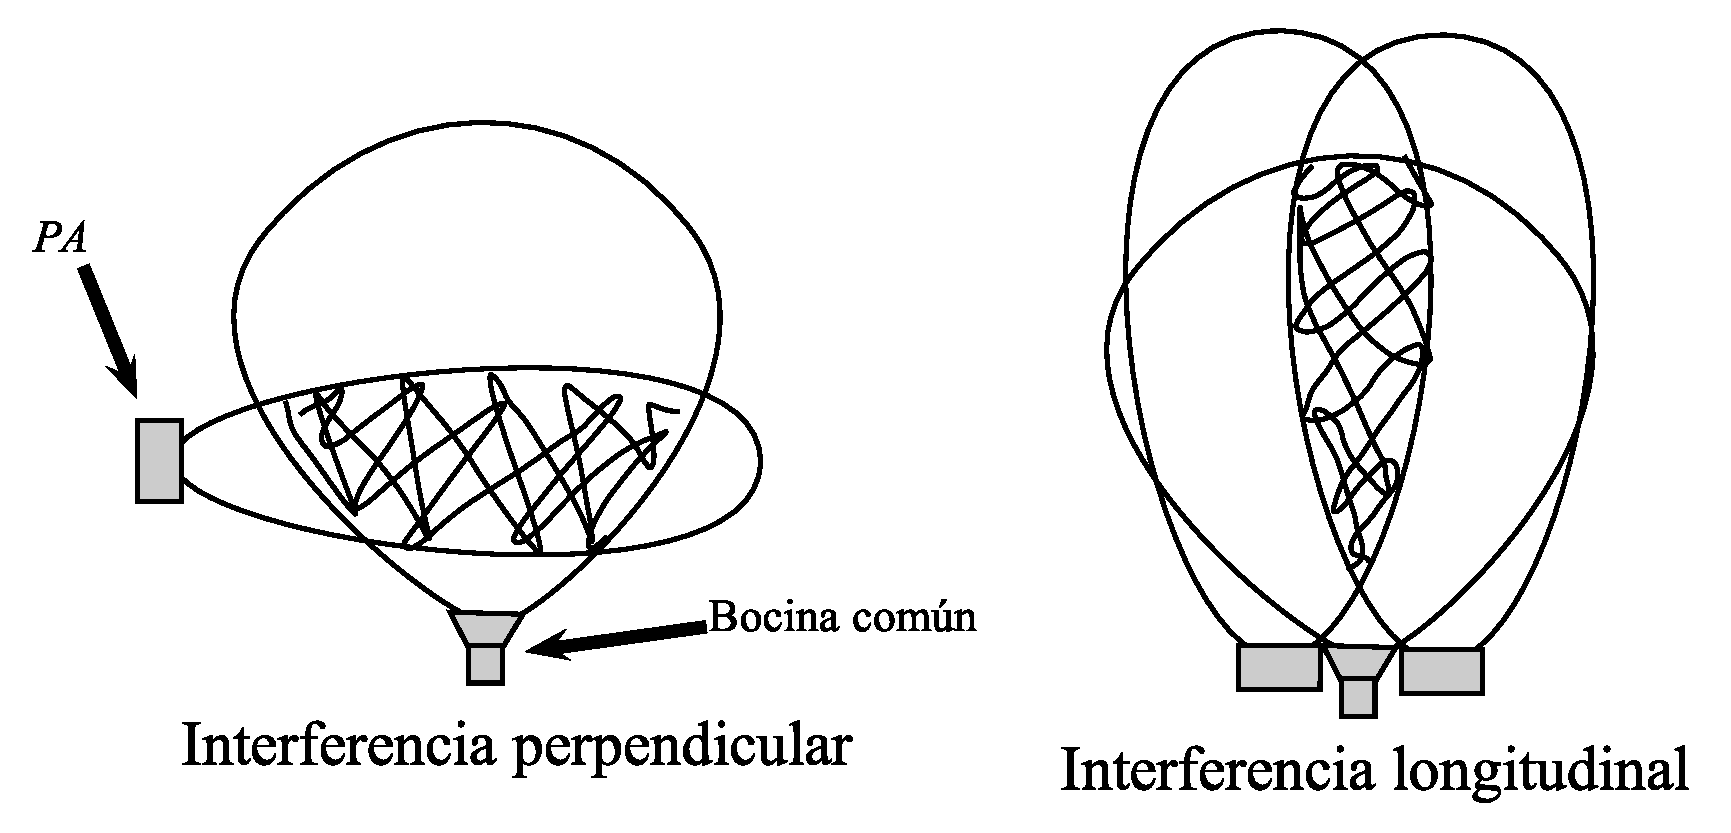
\includegraphics[scale=0.31]{introexp}
\caption{Caption for the image (Where did you get this?)}
\label{fig:introexp}
\end{figure}
Explain Figure \ref{fig:introexp} properly. 
%---------------------------------
%
% --------------------------------
\chapter{La ecuación de Khokhlov–Zabolotskaya–Kuznetsov}\label{chapter.kzk}

\begin{align}
\tildeps\left( \frac{\partial^2}{\partial x_1^2} +\frac{\partial^2}{\partial y_1^2}\right)p +\frac{1}{c_0^2}\frac{\partial^2p}{\partial \tau^2} - \frac{1}{c_0^2}\frac{\partial^2p}{\partial \tau^2} - \tildeps \frac{2}{c_0}\frac{\partial^2p}{\partial z_1\partial \tau}+ \frac{\delta}{c_0^4}\frac{\partial^3p}{\partial \tau^3} = -\frac{\beta}{\rho_0 c_0}\frac{\partial^2p^2}{\partial \tau^2}\text{,}\nonumber \\
-\frac{c_0}{2}\times\left[\tildeps\left( \frac{\partial^2}{\partial x_1^2} +\frac{\partial^2}{\partial y_1^2}\right)p - \tildeps \frac{2}{c_0} \frac{\partial^2p}{\partial z_1\partial \tau}+
\frac{\delta}{c_0^4}\frac{\partial^3p}{\partial \tau^3}\right]  = -\frac{c_0}{2}\times\left[-\frac{\beta}{\rho_0 c_0}\frac{\partial^2p^2}{\partial \tau^2}\right] \label{eqn:prekzk}\text{.}
\end{align}
%
...

%---------------------------------
%
%---------------------------------
%
%---------------------------------
\chapter{Conclusiones}
\begin{flushright} 
I was sick - sick unto death with that long agony...\\
\emph{- The Pit and the Pendulum-}\\
\emph{Edgar Allan Poe}
\end{flushright}

Este trabajo consistió en la modelación matemática, así como la construcción de una bocina direccional. Partiendo desde las ecuaciones básicas de la acústica, y con base en un esquema de orden apropiado y sólido, se construyó la ecuación de onda que describe los fenómenos de difracción, absorción y no linealidad (la ecuación KZK). A partir de ahí, los supuestos apropiados fueron adoptados para terminar con un modelo que sirviera para simular el fenómeno y tener un marco de referencia; pues la siguiente parte del trabajo consistió en la experimentación sobre el fenómeno.\medskip\\
Como cierre para el trabajo, se exhiben los comentarios acerca de los experimentos realizados en el capítulo anterior. ...
\section{Comment on your Results.} 
El trabajo consistió en el desarrollo de un modelo que explicara la interacción no lineal en el campo cercano de las ondas ultrasónicas (de AM), hasta el modelo KZK que describe de forma precisa la propagación sonora que considera los efectos de difracción, absorción y no linealidad del medio.
\subsection{Experimentos sobre la funcionalidad común del PA}
Para los primeros experimentos, se pudo observar que, a pesar de que las mediciones no se hicieron en una cámara anecóica, éstas se muestran bastante cercanas a las predicciones hechas en las simulaciones. La figura ....
\subsection{Experimentos de cancelación sonora}
Estos experimentos, no pretendían establecer un sistema de control de ruido como el mostrado en \cite{feasibility}, sino buscar algún indicio de que existe algún tipo de interacción entre las ondas ultrasónicas y las audibles. Los experimentos realizados en esta etapa fueron mucho más sensibles al ruido externo, y las condiciones no ideales fueron determinantes en el resultado, por lo menos de los experimentos de interacción de las ondas con varias frecuencias....
\section{Aplications of your work}
Las aplicaciones de la acústica no lineal no se limitan al desarrollo de un arreglo paramétrico. Como se vio en el capítulo \ref{chapter.pa}, éste es únicamente una aplicación derivada de una condición muy específica del medio en el que se trabaja. El rango de aplicaciones derivadas de la acústica no lineal, y en particular los usos que tiene la ecuación KZK, es muy amplio y depende en gran parte de ...
\subsubsection{Ethics ?? }
Es claro que el progreso científico no debe estar exento de la responsabilidad de advertir sobre las consecuencias del mal manejo de las tecnologías desarrolladas. En el caso presentado en este trabajo, e....
\section{Future work}
El trabajo desarrollado en esta tesis tiene una trayectoria hacia el futuro muy bien definida y con un alto potencial de desarrollo. En términos del estudio del arreglo paramétrico en sus funcionalidades comunes,...
%---------------------------------

\newpage

% To make a glossary (not actually sure how...)
%\gloss[nocite]{*} \printgloss{glossary}

% command to update::
% makeindex -s baa_main.ist -t baa_main.glg -o baa_main.gls baa_main.glo

\newpage

% If you need it to say anything other than "Appendix"
%\addcontentsline{toc}{chapter}{Appendix}
% \appendix
% \chapter{Acotamiento de los parámetros $(\eta, \epsilon)$}\label{app3}


\begin{table}[hbpt]
\small
\centering
\caption{Rangos de parámetros en el aire}
\begin{tabular}{cccc}
\hline
Temperatura [$^{\circ}$C]& Viscosidad, $\mu$ [Pa] & Velocidad, $c_0$ $[m/s]$& Densidad, $\rho_0$ $[kg/m^3]$\\
\hline
35 & 1.605$\times 10^{-5}$ & 351.88 & 1.1455 \\
30 & 1.632$\times 10^{-5}$ & 349.02 & 1.1644 \\ 
25 & 1.658$\times 10^{-5}$ & 346.13 & 1.1839 \\ 
20 & 1.685$\times 10^{-5}$ & 343.21 & 1.2041 \\ 
15 & 1.711$\times 10^{-5}$ & 340.27 & 1.225 \\ 
10 & 1.736$\times 10^{-5}$ & 337.31 & 1.2466 \\ 
5 & 1.762$\times 10^{-5}$ & 334.32 & 1.2690 \\ 
0 & 1.787$\times 10^{-5}$ & 331.3 & 1.29220 \\ 
-5 & 1.812$\times 10^{-5}$ & 328.25 & 1.3163 \\ 
-10 & 1.837$\times 10^{-5}$ & 325.18 & 1.3413 \\ 
-15 & 1.862$\times 10^{-5}$ & 322.07 & 1.3673 \\ 
-20 & 1.886$\times 10^{-5}$ & 318.94 & 1.3943 \\ 
-25 & 1.910$\times 10^{-5}$ & 315.77 & 1.4224 \\ 
\hline
\end{tabular}
\label{tab:app3}
\end{table}

% \chapter{El parámetro $B\slash A$}\label{section.app.ba}


\newpage
% If you need it to say anything that is not "References"
%\addcontentsline{toc}{chapter}{Bibliografía}

\bibliographystyle{siam} % or alpha, IEEEtraN, ...
\bibliography{\myrefs} % you actually need a .bib file for this(Not included)
% you actually need a .bib file for this(Not included)
%
%
% YOU WILL NEED TO ADD THE BIB FILE HERE WITH YOUR REFERENCES.
% wE'LL DO THIS TOWARDS THE END WHEN YOU ACTUALLY HAVE A REPORT!!!
%
%
%
% % This is a template for a bibliography file in which you don't use BibTeX. This has its benefits
% and drawbacks, for one thing, BibTeX files (.bib) can be a lot more versatile, so think about 
% the size of your work, you might want to consider using this or a BibTeX file. 
% 
% The report template uses natbib, which allows you to use some pretty neat features of 
% citations in a simple way, through your .bib file. And the rerunpdf.sh is a simple script that 
% lets you compile everything in a single go. 

\begin{thebibliography}{9999}
% ----- Libros ------
\bibitem{edplectures} ~Arnold, Vladimir (2000) 
\emph{Lectures on Partial Differential Equations}, Springer.
\bibitem{fundaments} ~Blackstock, David (2000)
\emph{Fundamentals of Physical Acoustics}, \textsc{Wiley-Interscience}, John Wiley \& Sons.
\bibitem{feasibility} ~Brooks, Laura A.  Zander, Anthony C.  Hansen, Colin (2005)
\emph{Investigation into the feasibility of using a parametric array control source in an active noise control system.}, Proceedings of Acoustics, November 2005, 39-45.
\bibitem{milenio} ~Córdoba Gazolaz, Diego (2011)
\emph{Las ecuaciones de Navier-Stokes}, Jornadas sobre los problemas del milenio, Real Sociedad Matemática Española \url{garf.ub.es/milenio/}
\bibitem{woo2} ~Gan, Woon-Seng; Shi, Chuang (2010)
\emph{Development of a Parametric Loudspeaker: A novel directional sound generation technology}, IEEE Potentials, November/December 2010, 20-24.
\bibitem{woo1} ~Gan, Woon-Seng; Tan, Ee-Leng; ~Kuo, Sen M. (2011)
\emph{Audio Projection. Directional sound and its application in immersive communication}, IEEE Signal Processing Magazine, January 2011, 43-57.
\bibitem{nonlinear} ~Hamilton; Blackstock (2008)
\emph{Nonlinear Acoustics}, Acoustical Society of America.
\bibitem{hansen} ~Hansen, Colin \emph{Fundamentals of Acoustics}, Department of Mechanical Engineering, University of Adelaide, Australia.
\bibitem{construccion} ~Kazunori, Miura (2011)
\emph{Richtschall mit Ultraschall},  \textsc{Elektor}, Ausgabe 483, \url{http://www.elektor.de} (comunicación personal).
\bibitem{wikiviscosidad} ~Kim, You-Kae; ~Han, J.-G; ~Kim, Youn J.
\emph{Numerical Analysis on Flow Characteristics of an Atmospheric Plasma Touch}, Center for Advanced Plasma Surface Technology, Sungkyunkwan University.
\bibitem{opp} ~Oppenheim, Alan V.; ~Willsky, Alan S. ; ~Nawab, S. Hamid (1998)
\emph{Señales y Sistemas}, \textsc{Prentice Hall}, Seunda edición.
\bibitem{pierce} ~Pierce, Allan D. (1989)
\emph{Acoustics: An introduction to its physical principles and applications}, Acoustical Society of America.
\bibitem{pompel} ~Pompei, Joseph (1999)
\emph{The use of airborne ultrasonics for generating audible sound beams}, Journal of the Audio Engineering Society, Vol. 47, No. 9, 726-731.
\bibitem{pompeii} ~Pompei, F. Joseph (2002)
\emph{Sound from ultrasound: The Parametric Array as an Audible Sound Source}, Dissertation for the degree of Dpctor of Philosophy, Massachusetts Institute of Technology.
\bibitem{hankel} ~Poularikas, Alexander (2000)
\emph{The Transforms and Applications Handbook}, CRC Press LLC.
\bibitem{rae} ~Real Academia de la Lengua Española (2001). \emph{Diccionario de la lengua española}, 22$^{\circ}$ edición. Consultado en \url{rae.es}
\bibitem{mathkzk} ~Rozanova-Pierrat, Anna (2007)
\emph{The Kohkhlov-Zabolotskaya-Kuznetsov equation}, C.R Math. Acad. Sci. Paris, 344, no.5, 337-342.
\bibitem{datatransducer}~S. Square Enterprise Company Limited,  Pro-Wave Electronics Corporation 
\emph{Air Ultrasonic Ceramic Transducers: DATASHEET}. \url{www.pro-wave.com.tw}
\bibitem{shure} Shure Brothers Incorporated. (1995)
\emph{Miniature Gooseneck-mounted supercardioid condenser microphone}, \textsc{Model SM99 User Guide}.
\bibitem{numericalkzk} ~Yang-Sub, Lee (1993), 
\emph{Numerical Solution of the KZK equation for pulsed finite amplitude sound beams in thermoviscous fluids}, Dissertation for the degree of Doctor of Philosophy, University of Austin Texas.
\bibitem{fujimoto} ~Yonehama, Masahide; ~Fujimoto, Jun-ichiroh; ~Kawamo, Yu; ~Sasabe, Shoichi (1983)
\emph{The audio spotlight: An application of nonlinear interaction of sound waves to a new type of loudspeaker design}, Journal of Acoustical Society of America, Vol. 73, No. 5, May 1983, 1532-1536.
\bibitem{westervelt} ~Westervelt, Peter (1962)
\emph{Parametric Acoustic Array}, Journal of Acoustical Society of America, Vol. 35, No. 4, 535-537.
\bibitem{wikivelocidad} ~Wikipedia: The Free Encyclopedia (2013).
\emph{Speed of Sound: Details},  Wikimedia Foundation Inc. disponible en \url{http://en.wikipedia.org/wiki/Speed_of_sound} (consultada 16 de octubre de 2013).
\bibitem{factors} ~Zhang, Yang; Tao, Limin (2011)
\emph{Factors analysis of the sound field for audio directional systems}, 2011 International Conference on Electronic \& Mechanical Engineering and Information Technology, 12-14 August, 758-761.

\end{thebibliography} % We provided this, but it shouldn't be done this peasant way!

\end{document}
